\documentclass[11pt]{article}
\usepackage[margin=25mm]{geometry}
\usepackage{amsmath}
\usepackage{tikz}
\usetikzlibrary{arrows.meta,positioning}
\definecolor{demoBlue}{HTML}{3478D4}
\tikzset{point/.style={circle,fill=demoBlue,inner sep=2pt}}
\title{A Few Vector Sketches}
\author{Mathlidelux Demo}
\date{}
\begin{document}
\maketitle
\section{A triangle}
A synthetic drawing with three labeled vertices.
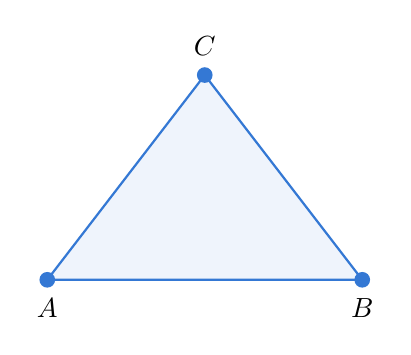
\begin{tikzpicture}[thick]
  \draw[demoBlue,fill=demoBlue!8] (0,0) -- (4,0) -- (2,2.6) -- cycle;
  \node[point,label=below:$A$] at (0,0) {};
  \node[point,label=below:$B$] at (4,0) {};
  \node[point,label=above:$C$] at (2,2.6) {};
\end{tikzpicture}

The area is $S=bh/2$.
\section{A workflow}
\begin{figure}[ht]
\centering
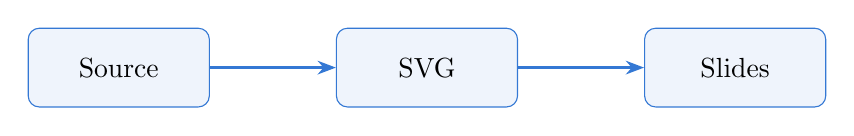
\begin{tikzpicture}[node distance=16mm,box/.style={draw=demoBlue,fill=demoBlue!8,rounded corners,minimum height=10mm,minimum width=23mm}]
  \node[box] (a) {Source};
  \node[box,right=of a] (b) {SVG};
  \node[box,right=of b] (c) {Slides};
  \draw[-{Stealth},thick,demoBlue] (a) -- (b);
  \draw[-{Stealth},thick,demoBlue] (b) -- (c);
\end{tikzpicture}
\caption{A fictional workflow used for demonstration.}
\end{figure}
\end{document}
